\documentclass[12pt,twoside,spanish,a4paper]{book}\usepackage[]{graphicx}\usepackage[]{color}
% maxwidth is the original width if it is less than linewidth
% otherwise use linewidth (to make sure the graphics do not exceed the margin)
\makeatletter
\def\maxwidth{ %
  \ifdim\Gin@nat@width>\linewidth
    \linewidth
  \else
    \Gin@nat@width
  \fi
}
\makeatother

\definecolor{fgcolor}{rgb}{0.345, 0.345, 0.345}
\newcommand{\hlnum}[1]{\textcolor[rgb]{0.686,0.059,0.569}{#1}}%
\newcommand{\hlstr}[1]{\textcolor[rgb]{0.192,0.494,0.8}{#1}}%
\newcommand{\hlcom}[1]{\textcolor[rgb]{0.678,0.584,0.686}{\textit{#1}}}%
\newcommand{\hlopt}[1]{\textcolor[rgb]{0,0,0}{#1}}%
\newcommand{\hlstd}[1]{\textcolor[rgb]{0.345,0.345,0.345}{#1}}%
\newcommand{\hlkwa}[1]{\textcolor[rgb]{0.161,0.373,0.58}{\textbf{#1}}}%
\newcommand{\hlkwb}[1]{\textcolor[rgb]{0.69,0.353,0.396}{#1}}%
\newcommand{\hlkwc}[1]{\textcolor[rgb]{0.333,0.667,0.333}{#1}}%
\newcommand{\hlkwd}[1]{\textcolor[rgb]{0.737,0.353,0.396}{\textbf{#1}}}%
\let\hlipl\hlkwb

\usepackage{framed}
\makeatletter
\newenvironment{kframe}{%
 \def\at@end@of@kframe{}%
 \ifinner\ifhmode%
  \def\at@end@of@kframe{\end{minipage}}%
  \begin{minipage}{\columnwidth}%
 \fi\fi%
 \def\FrameCommand##1{\hskip\@totalleftmargin \hskip-\fboxsep
 \colorbox{shadecolor}{##1}\hskip-\fboxsep
     % There is no \\@totalrightmargin, so:
     \hskip-\linewidth \hskip-\@totalleftmargin \hskip\columnwidth}%
 \MakeFramed {\advance\hsize-\width
   \@totalleftmargin\z@ \linewidth\hsize
   \@setminipage}}%
 {\par\unskip\endMakeFramed%
 \at@end@of@kframe}
\makeatother

\definecolor{shadecolor}{rgb}{.97, .97, .97}
\definecolor{messagecolor}{rgb}{0, 0, 0}
\definecolor{warningcolor}{rgb}{1, 0, 1}
\definecolor{errorcolor}{rgb}{1, 0, 0}
\newenvironment{knitrout}{}{} % an empty environment to be redefined in TeX

\usepackage{alltt}
\usepackage{geometry}\geometry{top=3cm,bottom=3cm,left=3cm,right=3cm}
\usepackage{fancyhdr}
\usepackage{amssymb}
\usepackage{amsmath}
\usepackage{url}
%\usepackage{mathrsfs}
\usepackage{longtable}
\usepackage{tocbibind}
\usepackage{titlesec}
\usepackage{makeidx}
\usepackage{boxedminipage}
\usepackage[utf8]{inputenc}
%\usepackage[all,2cell,dvips]{xy}
\usepackage{graphicx}
\usepackage{float}
\usepackage[spanish,es-tabla]{babel}
%\usepackage{parskip}
%\usepackage{multirow}
%\usepackage{multicol}
\usepackage{verbatim}
%\usepackage{fancyvrb}
\usepackage[authoryear]{natbib}

\fancyhf{} 
\fancyhead[LE]{\leftmark} 
\fancyhead[RO]{\nouppercase{\rightmark}} 
%\fancyfoot[LE,RO]{\thepage} 
\rfoot{\thepage} 
\pagestyle{fancy} 

\topmargin 2mm
\oddsidemargin 2mm
\evensidemargin 2mm

\makeindex
\setcounter{secnumdepth}{3}

\linespread{1.6}
\IfFileExists{upquote.sty}{\usepackage{upquote}}{}
\begin{document}





\pagenumbering{roman}

%%%%%%%%%%%%%%%%%%%%%%%%%% CARATULA %%%%%%%%%%%%%%%%%%%%%%%%%%%%%%%%%%%%%%%%%%
\thispagestyle{empty}

\begin{center}


\includegraphics[width=0.20\textwidth]{img/udelar_logo.jpg}



UNIVERSIDAD DE LA REPÚBLICA

Facultad de Ciencias Económicas y de Administración

Licenciatura en Estadística

Informe de Pasantía

\vspace{2.5cm}


\textbf{\large Estimación en dominios de indicadores socioeconómicos a partir de la Encuesta Continua de Hogares}

\vspace{1.5 cm}

\textbf{Mauricio Pittamiglio}


\end{center}


\vspace{2cm}

\noindent Tutores:\\
\noindent Ignacio Alvarez-Castro\\
\noindent Juan José Goyeneche\\


\vspace{1cm}

\begin{center}

\noindent Montevideo, Fecha.

\end{center}

%%%%%%%%%%%%%%%%%%%%%%%%%%%%%%%%%%%%%%%%%%%%%%%%%%%%%%%%%%%%%%%%%%%%%%%%%%%%%%%%%%%

\tableofcontents

%%%%%%%%%%%%%%%%%%%%%%%%%%%%%%%%%%%%% RESUMEN %%%%%%%%%%%%%%%%%%%%%%%%%%%%%%%%%%%%%%%%%%%

% 'resumen.Rnw'

%%%%%%%%%%%%%%%%%%%%%%%%%%%%%%%%%%%%%%%%%%%%%%%%%%%%%%%%%%%%%%%%%%%%%%%%%%%%%
\listoffigures
\listoftables


\setcounter{page}{1} 
 
\pagenumbering{arabic}

%%%%%%%%%%%%%%%%%%%%%%%%% INTRODUCCION %%%%%%%%%%%%%%%%%%%%%%%%%%%%%%%%%%%%%%%%%%
\chapter{Introducción \label{cap:Intro}}

El objetivo de este trabajo es generar una herramienta computacional que facilite el procesamiento de la Encuesta Continua de Hogares (ECH) mediante el cálculo de diversos indicadores y sus respectivos intervalos de confianza, aportando además una visualización interactiva de los resultados.

Las encuestas por muestreo no solo son utilizadas para obtener estimaciones a nivel de toda la población, sino que también pueden ser útiles para realizar estimaciones en subconjuntos de la población. Estos subconjuntos son denominados dominios, y los mismos pueden estar definidos por áreas geográficas, grupos demográficos u otro tipo de subpoblaciones.

Se trabajará con distintos indicadores socioeconómicos que se obtienen a partir de estimaciones provenientes de la Encuesta Continua de Hogares. Año a año el Instituto Nacional de Estadística (INE) hace públicas las bases de datos de la encuesta junto con un informe donde se presentan los resultados de distintos indicadores, en su mayoría a nivel nacional y desagregando en Montevideo e interior. En este trabajo se busca extender la cantidad de indicadores incluyendo desagregaciones departamentales en todos ellos.

Los indicadores presentados en este trabajo abordan distintas dimensiones, como ser, educación, salud, mercado laboral, entre otras. Estos se calculan tanto a nivel de toda la población (total país), así como para distintas aperturas (dominios o áreas de estimación), las cuales son definidas a nivel geográfico (departamentos). Algunos de estos indicadores son un insumo clave para la economía de los países y por ende para la toma de decisiones de las políticas públicas.

Como experiencia personal trabajé con la ECH, principalmente con el cálculo de indicadores a partir de esta encuesta, y contar con una herramienta como la realizada en este trabajo simplifica mucho la tarea. 

Otra de las ventajas de esta aplicación es la disponibilidad en la web y el no necesitar de conocimientos en R o en algún otro programa estadístico para poder obtener las estimaciones puntuales e intervalos de confianza para los indicadores, pudiendo visualizar interactivamente los resultados a partir de tablas o distintos gráficos.

Este trabajo se estructura de la siguiente manera.

En el capítulo 2 se presentan los métodos estadísticos utilizados en este trabajo, tanto los conceptos como las fórmulas que se aplican tanto en las estimaciones puntuales como para los errores estándar e intervalos de confianza. En el capítulo 3 se define el diseño de la ECH y se presentan los indicadores trabajados. El capítulo 4 refiere a la computación estadística, explicando la forma de cálculo de los indicadores, las características y el funcionamiento de la aplicación. En el capítulo 5 se presenta un ejemplo de aplicación de la app en dos indicadores. Finalmente en el capítulo 6 se realiza la discusión final, presentando los posibles trabajos a futuro.

\chapter{Métodos estadísticos \label{cap:Met}}

\section{Introducción \label{sec:in}}

Todos los indicadores presentados en este trabajo son estimaciones, por lo tanto se encuentran sujetas a errores de muestreo por el hecho de ser obtenidas a partir de una parte de la población (muestra) y no a partir de un censo. Estos errores de muestreo dependen de varios factores como ser: la variabilidad de la variable de interés, el tipo de indicador (parámetro), el dominio de estimación, la estrategia de selección de la muestra (diseño muestral) y los ajustes realizados para la construcción de los ponderadores.

El error de muestreo de la estimación de un parámetro es generalmente cuantificado por medio del error estándar de la estimación, que mide la variación de las estimaciones entre las distintas muestras y es el insumo principal para la construcción de intervalos de confianza.

Existen también los errores no muestrales, estos no se deben a la utilización de una muestra, sino a otras causas, como errores en la recolección o en el procesamiento de los datos, entre otros. Estos no serán abordados en este trabajo en particular.

En su mayoría los indicadores presentados son ratios (tasas, promedios y proporciones).

\subsection{Dominios \label{subsec:dom}}

En la práctica, las encuestas nacionales como la ECH, no son solamente utilizadas para hacer estimaciones a nivel de toda la población sino que también se realizan para diferentes subpoblaciones. Estas subpoblaciones para las cuales se computan de manera específica, tanto estimaciones puntuales como intervalos de confianza, son denominadas dominios \citep{sarndal2003model}.

En \citep{rojas2016estrategias} se introduce la siguiente definición de dominios.

\newtheorem{defi}{Definición}[chapter]

\begin{defi}
Un dominio $U_d$ es una sub-población específica o subgrupo poblacional que cumple las siguientes condiciones: 
\begin{enumerate}
\item $U_d \subset U$, tal que $U=\bigcup_{d=1}^{D}U_d$
\item Si $k \in  U_l$, entonces $k \notin  U_d$ para $d \neq l$
\item El número de elementos en el dominio $U_d$ es $N_d$ y es llamado tamaño absoluto del dominio.
\item La proporción de elementos en el dominio $U_d$ con respecto al tamaño poblacional es $P_d =\frac{N_d}{N}$ y se conoce como tamaño relativo del dominio.

\end{enumerate}
\end{defi}

Los dominios pueden clasificarse como planeados o no planeados. Los dominios planeados son aquellas subpoblaciones para las cuales se quiere brindar estimaciones con precisiones específicas y los mismos son definidos como estratos de diseño, lo cual permite definir tamaños de muestra específicos. Mientras que los dominios no planeados, son aquellos que no fueron tenidos en cuenta a la hora de diseñar la muestra, debido a que generalmente no se tiene información en el marco de muestreo. Estos dominios son los más comunes en la práctica y un claro ejemplo de los mismos son aquellos definidos por las personas que se encuentran comprendidas dentro de un tramo de edad específico.

\section{Estimaciones puntuales \label{sec:estpunt}}

En toda encuesta por muestreo, el objetivo es seleccionar una muestra aleatoria $s$ de tamaño $n$ de una población $U$ de tamaño $N$. Utilizando la muestra aleatoria $s$ se busca obtener estimaciones de distintos parámetros de interés de la población $U$. Un parámetro de interés puede ser el total de la variable de interés $y$, el cual viene dado por:

\[ t=\sum_{i=1}^{N}y_{i}=\sum_{i\in U}^{}y_{i} \]

La mayoría de los indicadores calculados en este trabajo se obtienen a partir del cociente (ratio) entre totales de dos variables $y$ y $z$, quedando definido de la siguiente manera:

\[ R=\frac{\sum_{i\in U} y_i}{\sum_{i\in U} z_i} \]

Las unidades, tanto hogares como personas, tienen una probabilidad de inclusión que viene determinada por el diseño muestral utilizado, la cual se denota como:

\[ \pi_i=\text{Prob} (i \in s) \]

Posteriormente, la probabilidad de inclusión $\pi_i$ de una unidad $i$ en la muestra $s$ es utilizada como insumo principal para calcular los ponderadores. El ponderador $w$ de una unidad (hogar o persona) incluida en la muestra se define como el inverso de la probabilidad de selección $\pi_i$, es decir:

\begin{equation}\label{m4}
\begin{array}{cc}
w_i=\frac{1}{\pi_i}
\end{array}
\end{equation}

El ponderador $w_i$ indica cuántas unidades de la población $U$ que no fueron seleccionadas representa la unidad $i$ que fue encuestada, es decir que pertenece a la muestra $s$.

Para poder computar las estimaciones de los parámetros de interés, se define el estimador de Horvitz-Thompson.

\[ \hat{t}_{\pi }=\sum_{s}^{}\frac{y_{i}}{\pi _{i}} \]

El mismo también puede ser planteado de la siguiente forma:

\begin{equation}\label{m6}
\begin{array}{cc}
\hat{t}_{\pi }=\sum_{s}^{}w_i \times y_i
\end{array}
\end{equation}

Este estimador es insesgado para el total $t=\sum_{U}^{}y_i$. \citep{sarndal2003model} (CITAR SARNDAL POR LA DEMOSTRACIÓN). Por otra parte, el estimador de ratio o cociente $R$ entre dos variables queda definido:

\begin{equation}\label{m7}
\begin{array}{cc}
\hat R=\frac{\sum\nolimits_{i\in s} w_i \times y_i}{\sum\nolimits_{i\in s} w_i\times z_i}
\end{array}
\end{equation}

El estimador $\hat R$ es un estimador no lineal ya que es un cociente entre dos estimadores, por lo tanto es aproximadamente insesgado. En toda encuesta suelen existir problemas de no respuesta y/o cobertura, es decir, el marco de muestreo donde físicamente es seleccionada la muestra no tiene un enlace perfecto con la población. Esto implica que en la práctica no se utilizen de forma directa los ponderadores para realizar las expansiones, sino que estos son ajustados por no respuesta y posteriormente calibrados a información conocida de la población. Estos nuevos ponderadores ajustados son los que finalmente son utilizados para la producción de las estimaciones de los distintos indicadores (parámetros) y son los que se encuentran incluidos en las bases de datos públicas de la ECH.  (CITAR INFORME OPP?)

Generalmente, los ajustes por no respuesta tienden a aumentar el error estándar (SE) de las estimaciones, ya que buscan únicamente reducir el posible sesgo ocasionado por las unidades que no respondieron a la encuesta, mientras que por otro lado, la calibración busca reducir los SE por medio de variables auxiliares o de control que se encuentran correlacionadas con las variables de interés de la encuesta. 


\section{Estimación de los errores estándar (SE) \label{sec:estse}}

Como la muestra es aleatoria, los estimadores son variables aleatorias y están, por lo tanto, sujetos a fluctuación. Esta fluctuación puede ser medida a partir del error estándar de la estimación. El SE es una medida de la precisión de la estimación y la misma puede ser utilizada para realizar inferencia de la población de interés por medio de la construcción de intervalos de confianza. El SE cuantifica la variación entre las estimaciones obtenidas entre las distintas muestras. Son calculados con el objetivo de añadir a las estimaciones puntuales una medida de calidad de las mismas. Por lo tanto, el problema se encuentra en poder obtener una estimación del SE que refleje, en lo posible, todas las fuentes de variabilidad del estimador o al menos las más importantes. Las fuentes de variabilidad vienen dadas por el diseño muestral implementado, así como también los distintos ajustes que son llevados a cabo para obtener los ponderadores finales $w_i$.

En la práctica muchos usuarios que utilizan la bases de datos de encuestas públicas para realizar sus propias inferencias no siempre tienen en cuenta todas las fuentes de variabilidad que afectan al error estándar. Esto, puede derivar en la realización de inferencias inválidas sobre los parámetros de la población. Uno de los motivos por los cuales surge este problema es el no contar con los insumos necesarios en la bases de datos públicas de las encuestas sobre el diseño de muestreo. En el caso de la ECH, para los años anteriores a 2018 no se cuenta con la disponibilidad de información clave sobre el diseño muestral como los son las unidades primarias de muestreo (UPM) y los estratos a los que pertenece cada individuo.

Para un diseño complejo como el de la ECH, no existen métodos exactos para calcular los SE, lo que implica que se deba recurrir a distintas estrategias o métodos que aproximan de mejor forma la variabilidad de las estimaciones. Dentro de la amplia gama de métodos que existen se optó por el método del último conglomerado en conjunto con la linearización de Taylor para computar los SE, que es el más usado en la práctica y se encuentra implementado en el paquete \textit{survey} \citep{survey} del \textit{R} \citep{r}. Este método puede manejar tanto parámetros lineales como no lineales. (PAPER DE LUMLEY EXPLICA COMO FUNCIONA EL SURVEY) \citep{surveyLumley}.

\subsection{Método del último conglomerado \label{subsec:ultcong}}

El método del último conglomerado es utilizado ampliamente en la práctica para la estimación de los SE en diseños por conglomerados en una o varias etapas de selección, en donde, los conglomerados (UPM) son seleccionados con probabilidades proporcional al tamaño. 

A continuación se desarrolla el método del último conglomerado aplicado a un muestreo aleatorio, estratificado, por conglomerados y en dos etapas de selección, como lo es el de la ECH. Pero previamente, se introduce la notación y conceptos necesarios para desarrollar dicho método.

La población de interés $U$ es particionada en grupos o estratos $U_1, U_2,...,U_h,...,U_H$ excluyentes. En cada uno de los estratos, se selecciona una muestra aleatoria $s_h$ de forma independiente en dos etapas de selección. Sea $M_h$ la cantidad de UPM en el estrato $h$ y $N_h$ la cantidad de unidades en dicho estrato. En una primera etapa, dentro de un estrato $h$ se selecciona $m_h$ UPM entre las $M_h$ bajo un muestreo aleatorio sin reposición con probabilidad proporcional al tamaño en base a una medida de tamaño (MOS). La probabilidad de selección de la UPM $j$ perteneciente al estrato $h$ viene dada por:


 \[  \pi_{jh}=m_h\times \frac{\text{MOS}_j}{\sum\limits_{j=1}^{M_h}\text{MOS}_j} \] 

Luego, dentro de cada UPM $j$ seleccionada en la primera etapa dentro del estrato de diseño $h$, se seleccionan $n_{jh}$ unidades, generalmente, con igual probabilidad de selección bajo un muestreo aleatorio simple o sistemático con arranque aleatorio. La probabilidad de selección de la unidad $i$ dentro de la UPM $j$ viene dada por:

\[ \pi_{i|jh}=\frac{n_{jh}}{\text{MOS}_{j}} \]

La probabilidad de selección final de la unidad en la muestra queda definida de la siguiente forma:

\[ \pi_{ijh}=\pi_{jh}\times \pi_{i|jh} \]

Por lo que el peso muestral de la unidad $i$ queda definido como el inverso de la probabilidad de selección, es decir:

\[ w_{i}=\pi_{ijh}^{-1} \]

En la ECH, las UPM corresponden a conglomerados de zonas censales, mientras la medida de tamaño MOS para la definición de las probabilidades de inclusión, es el número de viviendas $N_j$ de la UPM $j$ según datos del último censo de población disponible (2011 en este caso). Finalmente, el número de viviendas en cada UPM seleccionada en la primera etapa es fijo, es decir $n_j=\alpha$. Bajo los dos criterios anteriores, las probabilidades de selección y por tanto los pesos muestrales son iguales dentro de un mismo estrato:

\[ \pi_{ijh}=\pi_{jh}\times \pi_{i|jh}=m_h\times \frac{N_j}{\sum\limits_{j=1}^{M_h}N_j}=\frac{m_h\times \alpha}{N_h}=\frac{n}{N} \]

Una vez definidos los ponderadores $w_i$, se pueden computar las estimaciones de los distintos indicadores. Sin embargo, el problema es que bajo este tipo de diseños no existen estimaciones insesgadas de los errores estándar, ya que el insumo principal para las estimaciones de los SE utilizando el estimador Horvitz-Thompson, son las probabilidades de inclusión de segundo orden, es decir, la probabilidad de que dos unidades cualquiera $i$ y $k$ pertenezcan a la muestra.

El método del último conglomerado asume que la mayor variabilidad en la estimación proviene de la primera etapa de muestreo, es decir, en la selección de las UPMs. Por lo tanto, la estimación del SE cuadrado (varianza) utilizando el método del último conglomerado para la estimación del total de una variable cualquiera $y$ para un muestreo aleatorio, estratificado, por conglomerados y en varia etapas de selección viene dada por:

\begin{equation}
\begin{array}{cc}
\widehat {\text{SE}}^2(\hat t)=\hat V (\hat t)= \sum\limits_{h=1}^H\frac{1}{m_h(m_h-1)}\times \sum\limits_{j \in s_h}(\hat t_{jh}\times m_h-\hat t_h)^2
\label{ec:m13}
\end{array}
\end{equation}

donde:

$m_h$ es la cantidad de UPM pertenecientes al estrato $h$ seleccionadas en la muestra.

$\hat t_{jh}=\sum\nolimits_{s_{jh}} w_i\times y_i$ es la estimación del total de la variable $y$ en la UPM $j$ perteneciente al estrato $h$.

$\hat t_h=\sum\nolimits_{h=1}^H\hat t_{jh}$ es la estimación del total de la variable $y$ en el estrato $h$.

Por otra parte, si el objetivo es estimar el total de la variable $y$ pero para un dominio o área de estimación cualquiera $d$, el SE se obtiene reemplazando en la ecuación anterior \ref{ec:m13} la variable $y$ por la variable $y_d$ la cual, toma el valor $y$ para los casos de la muestra incluidos en el dominio $d$ y cero en otro caso. Esta técnica se utiliza para añadir una variabilidad extra a las estimaciones, producto de que el tamaño de muestra en el dominio (por ejemplo, personas comprendidas en un determinado tramo de edad y dentro de un determinado departamento) es aleatorio. 


\subsection{Linearización de Taylor \label{subsec:taylor}}

La linearización de Taylor es un método ampliamente utilizado para aproximar SE de parámetros no lineales (como ser un ratio). La idea es aproximar un estimador no lineal por medio de una función lineal. Una vez realizado lo anterior y teniendo en cuenta el diseño muestral utilizado se obtiene una aproximación del SE del estimador. Para el caso del estimador de una tasa o ratio $R=t_y/t_z$, es aproximado utilizando el desarrollo de taylor de primer orden y dicha aproximación queda definida como:

\[ \hat  R \approx R +\frac{1}{t_z}\times \sum\nolimits_{i\in s} w_i\times (y_i-Rz_i) \]

Luego, el estimador de la varianza (o error estándar al cuadrado) se obtiene reemplazando la variable $y$ por una variable $r_i=y_i-\hat Rz_i$ y añadiendo el término $1/\hat t_z^{2}$.

\begin{equation}
\widehat {\text{SE}}^2(\hat R)=\hat V (\hat R)= \frac{1}{\hat t_z^2}\times\sum\limits_{h=1}^H\frac{1}{m_h(m_h-1)}\times \sum\limits_{j \in s_h}(\hat t_{r,jh}\times m_h-\hat t_{r,h})^2
\label{m15}
\end{equation}

donde:

$\hat t_z=\sum\nolimits_{i\in s}w_i\times z_i$ es la estimación del total de la variable $z$.

$\hat t_{r,jh}=\sum\nolimits_{s_{jh}} w_i\times r_i$ es la estimación del total de la variable $r$ en la UPM $j$ perteneciente al estrato $h$.

$\hat t_{r,h}=\sum\nolimits_{h=1}^H\hat t_{r,jh}$ es la estimación del total de la variable $r$ en el estrato $h$.

Al igual que para el caso de un total, el SE de la estimación de un ratio $R$ para un dominio $d$ se obtiene reemplazando en la ecuación \ref{m15} las variables $y$ y $z$ por sus correspondientes variables extendidas en el dominio, $y_d$ y $z_d$.

\section{Intervalos de confianza \label{sec:ic}}

A partir de la estimación de los errores estándar, se obtienen los intervalos de confianza. Estos son una medida de calidad de las estimaciones y son computados con el fin de poder extraer conclusiones sobre la población.

Los intervalos de confianza se suelen calcular de la siguiente manera:

\[ \hat \theta \pm \text{constante}\times \widehat{\text{SE}}(\hat \theta) \]

Donde el estimador $\hat \theta$ se asume tiene una distribución aproximadamente normal. Por lo que el intervalo de confianza para un parámetro cualquiera $\theta$ con un nivel de confianza $100(1-\alpha))\%$ queda definido como:

\[ \hat \theta \pm z_{1-\alpha/2}\times \widehat{\text{SE}}(\hat \theta) \]

Particularmente se trabajará con una confianza del $95\%$, por lo que al sustituir el valor de la constante:

\begin{equation}\label{m18}
\begin{array}{cc}
\hat \theta \pm 1.96\times \widehat{\text{SE}}(\hat \theta)
\end{array}
\end{equation}

Un intervalo con nivel de confianza del $95\%$ significa que, en promedio, de cada 100 muestras obtenidas bajo el mismo diseño, el intervalo contiene al verdadero valor del parámetro en 95 de ellas.

\chapter{Indicadores \label{cap:ind}}

\section{ECH \label{sec:ech}}

La Encuesta Continua de Hogares (ECH) es una encuesta realizada de forma ininterrumpida por el Instituto Nacional de Estadística (INE) desde el año 1968.  La ECH es un tema de interés nacional, ya que brinda los indicadores oficiales del mercado laboral y de ingresos de los hogares y las personas con periodicidad mensual, trimestral, semestral y anual, entre otros.

El diseño muestral de la ECH es aleatorio, estratificado, por conglomerados y en dos etapas de selección. Como primer paso para la selección de la muestra la población es particionada en estratos. El primer nivel es geográfico y corresponde a los diecinueve departamentos del país y a la zona metropolitana. En un segundo nivel, cada una de las localidades dentro del departamento es clasificada en cuatro categorías: i) localidades con más de 20.000 habitantes, ii) localidades entre 5.000 y menos de 20.000 habitantes, iii) localidades entre 200 y 5.000 habitantes y iv) áreas rurales y localidades con menos de 200 habitantes. Para Maldonado y Rocha se agrega un nivel más correspondiente a las zonas balnearias. En el departamento de Montevideo y zona metropolitana se conforman cinco y tres estratos socioeconómicos respectivamente.

Dentro de cada estrato y de forma independiente se selecciona, en una primera etapa, conglomerados de zonas censales (Unidades Primarias de muestreo - UPM) bajo un muestreo aleatorio, sistemático y proporcional al tamaño (PPS), utilizando como medida de tamaño (MOS) la cantidad de viviendas particulares según datos provenientes del último censo de población y vivienda del año 2011. Luego, en segunda etapa se seleccionan cinco viviendas titulares y dos viviendas suplentes en cada una de las UPM seleccionadas en la primera etapa, con igual probabilidad de selección bajo un muestreo aleatorio simple.

Dentro de cada vivienda seleccionada se relevan características propias de la vivienda así como del hogar que reside en la misma e información de todos los integrantes que conforman el hogar. Esto implica que la ECH brinde información para computar distintos indicadores no solo a nivel de hogar sino también a nivel de persona. Es por esto, que el INE publica dos bases de datos, una base con información a nivel del hogar y la vivienda y otra base con información a nivel de personas.

El tamaño de muestra efectivo anual de la ECH, es decir, la cantidad de hogares que cumplen los criterios de ser elegibles y respondieron se encuentra en el entorno de 42000 hogares.

Los datos de la muestra son ponderados, de forma de obtener estimaciones tanto a nivel nacional, departamental y de otros dominios de estudio, entre ellos, sexo y tramos de edades. Existen varias etapas para la determinación de los ponderadores finales de la ECH. El componente principal es el inverso de la probabilidad de selección del hogar y sus integrantes en la muestra de la ECH, denominado ponderador original. El ponderador original de un hogar perteneciente a un estrato cualquiera se define como el inverso de la tasa de muestreo en el estrato.

Los ponderadores originales son ajustados en varias etapas una vez concluida la recolección de la información. El primer ajuste se realiza en base a la no respuesta obtenida en campo, es decir, teniendo en cuenta las encuestas efectivamente realizadas. Un segundo ajuste se efectúa utilizando técnicas de calibración en base a las proyecciones de la población residente en viviendas particulares. Esto implica que la ECH expanda a la población proyectada para el año de referencia para cada uno de los departamentos del país, y para la estructura de la población a nivel del total del país por sexo y cinco tramos de edades (0 a 14 años, 15 a 29 años, 30 a 49 años, 50 a 64 años y 65 años o más). \citep{ine} (CITAR INFOME DEL INE)


\section{Listado de indicadores \label{sec:lista}}

Los indicadores presentados en este trabajo son calculados todos los años por el Observatorio Territorio Uruguay (OTU) perteneciente a la Oficina de Planeamiento y Presupuesto (OPP), y se encuentran disponibles en su página oficial. Estos indicadores se dividen en 7 categorías:

\begin{itemize}
\item Educación
\item Salud
\item Mercado laboral
\item Ingresos y bienestar
\item Tecnología y comunicación
\item Demografía
\item Viviendas y hogares

\end{itemize}

Dentro de la categoría \textit{Educación} se encuentran 17 indicadores, referidos a tasas de asistencia a distintos niveles educativos, tasas de analfabetismo, promedio de años de educación, entre otros.

En la categoría \textit{Salud} hay 3 indicadores que evalúan la afiliación a emergencias móviles y el tipo de atención en salud.

Hay 13 indicadores disponibles dentro de \textit{Mercado laboral}, además de los principales indicadores de este rubro (tasas de empleo, desempleo, actividad), se encuentran otros referidos a la informalidad, categoría de ocupación, entre otros.

La categoría \textit{Ingresos y bienestar} cuenta con 8 indicadores, índices de pobreza (en personas y hogares) y algunos indicadores presentes también en la categoría \textit{Mercado laboral} (empleo, desempleo e informalidad).

En \textit{Tecnología y comunicación} se encuentran 7 indicadores referidos a tenencia de distintos dispositivos como celulares o computadoras y a la utilización de estos dispositivos y de internet.

\textit{Demografía} contiene 3 indicadores referidos a residencias previas o lugar de nacimiento de las personas.

Finalmente la categoría \textit{Viviendas y hogares} cuenta con 8 indicadores, todos ellos referidos a distintas características de los hogares.

Recordando que hay indicadores que se encuentran en varias categorías, en total se trabaja con 53 indicadores socio-económicos, desagregando todos por departamento y a su vez hay algunos que se desagregan también por sexo o tramos etarios.

En anexo \ref{ane:ind} se presenta un listado completo de los indicadores trabajados.

\chapter{Métodos computacionales \label{cap:comp}}


\section{Estimación de los indicadores \label{sec:estindic}}

Para replicar el diseño muestral de la ECH y poder llevar a cabo el computo de los indicadores, se utiliza el software libre \textit{R}, más precisamente el paquete \citep{srvyr}. Este paquete utiliza las funciones del paquete \textit{survey} antes mencionado, permitiendo el uso de un estilo de sintaxis inspirado en el paquete \textit{dplyr} \citep{dplyr}.

Este paquete \textit{srvyr} cuenta con funciones tales como $survey\_mean$ para calcular medias o proporciones, $survey\_ratio$ para ratios o $survey\_total$ para totales. Estas funciones utilizan el valor que toma el indicador en cada uno de los individuos (hogares o personas según corresponda) de la muestra y los ponderadores, dando como resultado tanto las estimaciones puntuales que correspondan como las estimaciones de los errores estándar, utilizando las ecuaciones y metodologías descritas en este documento para realizar los cálculos.

A continuación se presenta un breve ejemplo de como se utilizan las funciones de esta librería, para el caso concreto del indicador \textit{Utilización de computadora el último mes por sexo}.

\begin{knitrout}
\definecolor{shadecolor}{rgb}{0.969, 0.969, 0.969}\color{fgcolor}\begin{kframe}
\begin{alltt}
\hlstd{pr}\hlkwb{<-}\hlstd{echP}\hlopt \hlkwd{as_survey_design}\hlstd{(}\hlkwc{ids}\hlstd{=upm_fic,} \hlkwc{weight}\hlstd{=pesoano}
                             \hlstd{,} \hlkwc{strata}\hlstd{=estrato)}

\hlstd{diseno}\hlkwb{<-} \hlstd{pr}
\hlstd{filtro}\hlkwb{<-} \hlstr{"e27>5"}
\hlstd{variable}\hlkwb{<-} \hlstr{"e61==1"}

\hlstd{ind}\hlkwb{<-}\hlstd{diseno}\hlopt
      \hlkwd{filter}\hlstd{(}\hlkwd{eval}\hlstd{(}\hlkwd{parse}\hlstd{(}\hlkwc{text}\hlstd{=filtro)))}\hlopt
      \hlkwd{group_by}\hlstd{(dpto, e26)}\hlopt
      \hlkwd{summarise}\hlstd{(}\hlkwc{estimacion.tot}\hlstd{=} \hlkwd{survey_mean}\hlstd{(}\hlkwd{eval}\hlstd{(}\hlkwd{parse}\hlstd{(}\hlkwc{text}\hlstd{=variable))))}
\end{alltt}
\end{kframe}
\end{knitrout}

En primer lugar se crea el objeto de diseño mediante la función $as\_survey\_design$, donde los insumos que se le indican son las unidades primarias de muestreo ($upm\_fic$), los ponderadores ($pesoano$) y los estratos ($estrato$). Todas estas son variables presentes en la base de datos de la ECH. Luego se crean los objetos filtro y variable, el filtro define la población objetivo que en este caso son las personas mayores de 5 años, mientras la variable utilizada es $e61==1$ la cual es una variable presente en la ECH que hace referencia a la utilización de computadora en el último mes.

Las líneas de código siguientes son la base de las funciones creadas para el cálculo de los indicadores, donde en este caso se le indica el objeto de diseño, se le aplica el filtro necesario, se agrupa por departamento y por sexo ($e26$) y se estima la media de la variable indicada para cada sexo a nivel de cada departamento, dando como resultado un objeto (data frame) con las estimaciones puntuales y errores estándar para el indicador deseado.

Tanto para el filtro como para la variable se utilizan las funciones $eval$ y $parse$, la función $parse$ convierte texto en expresiones, mientras la función $eval$ evalúa expresiones.

Para la simplificación del cálculo de los indicadores se crearon 9 funciones que varían dependiendo de los individuos involucrados (personas y hogares), la forma en la que se calcula cada indicador y las desagregaciones necesarias. Todas estas funciones estiman el indicador tanto a nivel de cada departamento como de todo el país y tienen como salida una tabla (data frame) con los resultados.

Todas las funciones necesitan de algunos insumos para estimar los indicadores correspondientes, estos son: 

\begin{itemize}
\item El diseño muestral.
\item El filtro a aplicar (de ser necesario). Este determina la población objetivo para la cual el indicador será calculado.
\item Variable(s) de interés: variable(s) necesaria(s) para el cálculo del indicador.
\item Vector con categorías de la variable de interés (en caso de ser necesario).

\end{itemize}

Las primeras 7 funciones se utilizan para los indicadores que se obtienen a partir de la base de personas de la ECH, mientras las últimas 2 trabajan con la base de hogares.

La \emph{funcion1} se utiliza para los indicadores que necesitan del cálculo de la proporción de individuos que cumplen determinada condición (por ejemplo quienes tienen estudios terciarios), desagregando además por sexo. 

La \emph{funcion2} es utilizada para los indicadores en los cuales es necesario calcular la proporción de distintas categorías de una variable, y también se desagrega por sexo. 

Las funciones \emph{funcion3}, \emph{funcion4} y \emph{funcion5} son similares, calculan proporciones al igual que en la función 1, pero desagregando en tramos de edad en lugar de por sexo. La diferencia entre estas tres funciones es que desagregan en distintos tramos etarios.

La \emph{funcion6} se utiliza unicamente para la estimación del indicador \textit{Promedio de años de educación de las personas de 25 años y más por sexo}. La variable en este caso es cuantitativa, se promedia y se desagrega por sexo.

La \emph{funcion7} se utiliza para los indicadores que hacen referencia a tasas brutas, es decir, necesitan del cálculo de un ratio.

Los indicadores \textit{Población total por condición de actividad por sexo} y \textit{Personas por tipo de atención en salud}, fueron calculados de manera particular, sin el uso de ninguna función.

Las funciones \emph{funcion8} y \emph{funcion9}, como se mencionó anteriormente, son las utilizadas para la estimación de los indicadores que se obtienen a partir de la base de hogares de la ECH. La \emph{funcion8} se utiliza para los indicadores que requieren el cálculo de la proporción de hogares que cumplen con determinada condición, mientras que en la \emph{funcion9}, la variable en cuestión presenta más de 2 categorías.

El indicador \textit{Hogares por tipo de relación con la vivienda} fue estimado de manera particular, sin el uso de ninguna función.

Se crean además funciones para el cálculo de los intervalos de confianza de las estimaciones, funcionando de la misma manera que las funciones mencionadas anteriormente pero obteniendo una salida diferente, 9 de ellas dan como salida una tabla con los extremos inferiores de los intervalos, mientras las otras 9 hacen lo mismo con los límites superiores.

El cálculo del indicador presentado anteriormente, una vez creadas las funciones, se reduce a la siguiente línea de código.

\begin{knitrout}
\definecolor{shadecolor}{rgb}{0.969, 0.969, 0.969}\color{fgcolor}\begin{kframe}
\begin{alltt}
\hlkwd{funcion1}\hlstd{(pr,}\hlstr{"e27>5"}\hlstd{,}\hlstr{"e61==1"}\hlstd{)}
\end{alltt}
\end{kframe}
\end{knitrout}

Este indicador es estimado en base a personas y con desagregación por departamento y por sexo. Se utiliza la función \textit{funcion1}, el diseño utilizado $pr$, el filtro $e27>5$ y la variable $e61==1$ son los presentados anteriormente.

\subsection{Descripción de los diseños \label{subsec:dis}}

El insumo \textit{diseño muestral} que utilizan las funciones creadas para el cálculo de los indicadores depende de la información disponible con la que cuente el usuario. En las bases públicas del INE no se cuenta con información del estrato ni de la UPM a la que pertenece el individuo, por lo que en la app aparecen dos opciones. La opción \textit{pública} se utiliza cuando no se cuenta con esta información, mientras que en caso de contar con esta se utiliza la opción \textit{estratos+UPM}.

En caso de no contar con la información de estratos y UPM, los cálculos de los intervalos de confianza son incorrectos, ya que esta información es esencial para poder realizar una aproximación correcta de los SE y así poder construir los intervalos de confianza.

Cabe aclarar que INE hizo pública esta información para los años 2018 y 2019.

\section{Aplicación web utilizando Shiny \label{sec:shiny}}

Shiny \citep{shiny} es una librería que permite crear fácilmente aplicaciones web interactivas a partir de R. La interactividad de estas aplicaciones permite la manipulación de los datos sin la necesidad de manipular el código, es decir, en caso de estar disponible en alguna página web, puede ser fácilmente utilizada por personas que no tengan conocimientos de R.

Estas aplicaciones cuentan con programación reactiva. Esto significa que al cambiar los valores de entrada (inputs) se volveran a ejecutar las partes del código de R correspondientes, lo que a su vez hará que se actualicen las salidas (outputs) modificadas, es decir, la modificación de un valor reactivo llevará automaticamente a todas las expresiones reactivas que dependen directa o indirectamente de este valor a ejecutarse nuevamente. 

Se cuenta además con widgets pre-construidos que facilitan la construcción de aplicaciones bonitas e interactivas. Un widget es un elemento web que los usuarios pueden interactuar con él enviando mensajes a la aplicación Shiny.

Una Shiny app contiene al menos dos componentes: un script para la interfaz del usuario (UI) donde se controla el diseño de la aplicación; y un script para realizar los cálculos necesarios (server). En el server se debe especificar como convertir los valores de entrada (inputs) en resultados (outputs).

\subsection{Monitor de indicadores socioeconómicos \label{subsec:app}}

Esta aplicación procesa los datos de la ECH, particularmente se realizó en base a la encuesta del año 2019, pero también funciona perfectamente para los años (..)2015 a 2018 y está pensada para que funcione también para los próximos años, en caso de que la encuesta no tenga cambios abruptos en su formato y estructura. Para el cálculo de los indicadores se utilizan un grupo de variables de la ECH, lo que hace a la app dependiente de esas variables, es decir, en caso de que esas variables cambien de nombre o dejen de estar disponibles, la app debe ser actualizada. Tanto en la aplicación como en los anexos \ref{ane:var} de este informe, estará disponible un listado con las variables utilizadas.

En esta aplicación en particular, previo a la creación del UI y el server, se cargan las librerías a utilizar, los datos espaciales necesarios para los gráficos de mapas, el listado de variables utilizadas de la ECH y se crean las funciones que se utilizan para el cálculo de los indicadores. Esta parte del código se corre solo una vez al iniciar la app.

\subsection{Interfaz del usuario \label{subsec:ui}}
La UI cuenta con tres partes, el encabezado (\textit{dashboardHeader}), la barra lateral (\textit{dashboardSidebar}) y el contenido (\textit{dashboardBody}).

Dentro del encabezado solo aparece el título y un link que lleva directamente a la página del INE donde están disponibles las bases de datos de la ECH.

La barra lateral es utilizada para cargar las bases de datos y para seleccionar la sección que se desee visualizar, ya sea la pestaña de introducción o las correspondientes a las diferentes categorías de los indicadores. Para cargar los datos se utiliza la función \textit{fileInput} y se deben cargar por separadas las bases de personas y de hogares de la ECH y el archivo que contiene la información acerca de los estratos y UPM (en caso de contar con el). También se incluye un widget mediante la función \textit{selectInput} para que el usuario pueda especificar si las bases utilizadas son las públicas o si se cuenta con la información de estratos y UPM.

\begin{figure}[htb]
\begin{center}
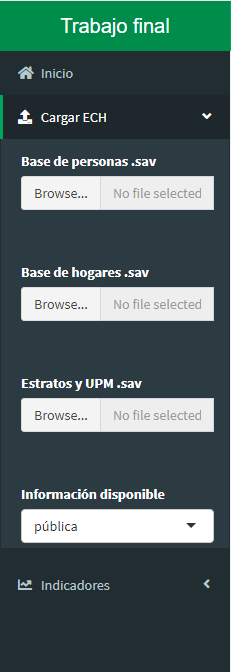
\includegraphics[width=0.30\textwidth]{img/Barra_lateral.PNG}
\caption{Barra lateral. \label{lateral}}
\end{center}
\end{figure}

En el body se especifica el contenido de cada una de las secciones. La ventana de inicio cuenta con dos pestañas, en la primera de estas se encuentra un manual de uso de la aplicación, donde se explica su utilidad y los pasos a seguir para el correcto funcionamiento de esta. Mientras en la segunda pestaña se encuentra un listado con las variables de las bases de datos de la ECH que son utilizadas en la app.

La sección de los indicadores cuenta con 3 pestañas (\ref{pest}).

\begin{figure}[h]
\begin{center}
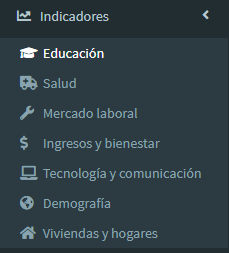
\includegraphics[width=0.30\textwidth]{img/cat.PNG}
\caption{Categorías de indicadores. \label{cat}}
\end{center}
\end{figure}

\begin{figure}[h]
\begin{center}

\includegraphics[width=0.30\textwidth]{img/pest.PNG}
\caption{Pestañas. \label{pest}}
\end{center}
\end{figure}

En la primera de estas pestañas se selecciona el indicador que se quiere calcular y se pueden visualizar dos tipos de gráficos para este indicador, un gráfico de mapa donde, en caso de que corresponda, se puede seleccionar la categoría a graficar, y un diagrama de barras (apiladas, agrupadas o simple según el caso). En la segunda pestaña se puede observar una tabla para las estimaciones puntuales del indicador seleccionado y un botón de descarga (\textit{downloadButton}) para poder descargar dicha tabla en formato csv. Mientras la tercer pestaña cuenta con las tablas para los límites de los intervalos de confianza de las estimaciones, divididas en dos paneles, uno para el límite inferior y otro para el superior, ambas tablas también cuentan con un botón de descarga.

\subsection{Comportamiento reactivo \label{subsec:server}}

La función server toma dos parámetros: \emph{input} y \emph{output}. El argumento \emph{input} es un objeto similar a una lista que contiene todos los elementos de entrada enviados por el navegador. Mientras el argumento \emph{output} es similar al anterior con la principal diferencia de que es usado para enviar objetos de salida y no para recibir objetos de entrada.

En esta parte del código se controla el comportamiento de la app. En primer lugar se crean todos los elementos reactivos (se guardan las bases de datos cargadas, los diseños y todos los indicadores) utilizando la función \textit{reactive}. Luego se crean todos los componentes de salida con funciones render, las tablas con \textit{renderDT} y los gráficos con \textit{renderPlotly}. Las funciones render cumplen con dos objetivos: establecer un contexto reactivo especial que rastrea automáticamente qué entradas usa la salida y convierte estas salidas del código de \emph{R} en \emph{HTML} adecuado para mostrar en una página web (CITAR MASTERING SHINY). Tanto las tablas como los gráficos se crean en outputs diferentes para cada una de las categorías de indicadores.

\textit{Plotly} \citep{plotly} hace los gráficos interactivos, cuenta con varias opciones para poder visualizarlos de manera más precisa y permite descargarlos como imagen.

\chapter{Ejemplo de aplicación \label{cap:aplic}}

En esta sección se presenta el procedimiento aplicado y los resultados obtenidos para el caso de dos indicadores en particular, la \texttt{tasa de desempleo por sexo} y \texttt{Hogares por presencia de lugar para cocinar}. Utilizando la ECH del 2019 y la información sobre los estratos y unidades primarias de muestreo (UPM).

\section{Tasa de desempleo \label{sec:desempleo}}

La tasa de desempleo es uno de los indicadores más importantes que brinda la ECH. El INE calcula este indicador todos los años a nivel departamental e incluso desagregando también por sexo.

Este indicador hace referencia a la proporción de personas desocupadas por sexo, donde, desocupada es toda persona que durante el período de referencia de la encuesta, no está trabajando por no tener empleo, que lo busca activamente, y están disponibles para empezar a trabajar. Se calcula como $\frac{Numero\; de\; personas\; desocupadas}{Poblacion \;Economicamente \;Activa}$.

Pasando al cálculo a partir de las funciones, el código es el siguiente:

\begin{knitrout}
\definecolor{shadecolor}{rgb}{0.969, 0.969, 0.969}\color{fgcolor}\begin{kframe}
\begin{alltt}
\hlkwd{funcion1}\hlstd{(pr,} \hlstr{"e27>13 & activo==1"}\hlstd{,} \hlstr{"desocupados==1"}\hlstd{)}
\end{alltt}
\end{kframe}
\end{knitrout}

Al ser un indicador calculado en base a personas, necesitando del cálculo de una proporción y desagregando por sexo se utiliza la \textit{funcion1}. El diseño utilizado es \textit{pr}, el fitro $e27>13$ y $activo==1$ indica que se calcula para los mayores de 13 años y la variable $activo==1$, es una variable creada a partir de otras variables de la ECH, que toma valor 1 cuando el individuo pertenece a la población económicamente activa. Finalmente la variable utilizada es $desocupados==1$ la cual también es una variable creada a partir de otras variables de la ECH y toma valor 1 cuando el individuo está desocupado y 0 si no lo está.

Para la obtención de los resultados de este indicador en la app en primer lugar se cargan las bases de datos necesarias, disponibles en la página web del INE. Primero se debe cargar la base de personas, luego la de hogares y en tercer lugar, el archivo con la información sobre estratos y UPM.

\begin{figure}[H]
\begin{center}
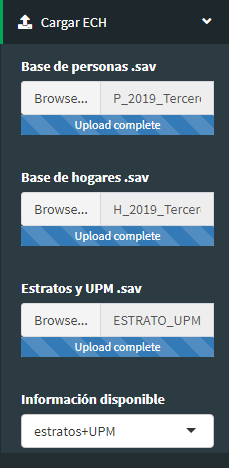
\includegraphics[width=0.30\textwidth]{img/bases.PNG}
\caption{Bases de datos. \label{pest}}
\end{center}
\end{figure}

Una vez cargadas las bases se selecciona dentro de la sección de indicadores, la categoría \textit{Mercado laboral} donde se encuentra este indicador. Una vez dentro de esta sección, se selecciona el indicador que se desea obtener, tal como se muestra en la figura \ref{ind}.

\begin{figure}[ht]
\begin{center}
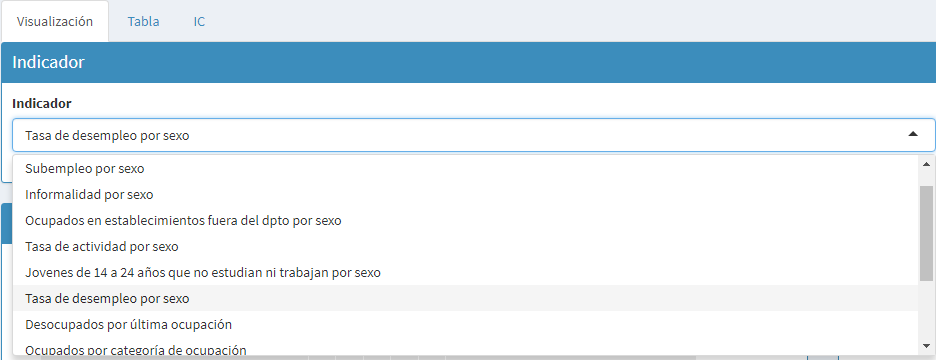
\includegraphics[width=1\textwidth]{img/indicador.png}
\caption{Selección del indicador Tasa de desempleo por sexo. \label{ind}}
\end{center}
\end{figure}

En la misma pestaña se observan como resultados los dos tipos de gráficos antes mencionados, los cuales se presentan en las figuras \ref{barras} y \ref{mapa}.

\begin{figure}[h]
\begin{center}
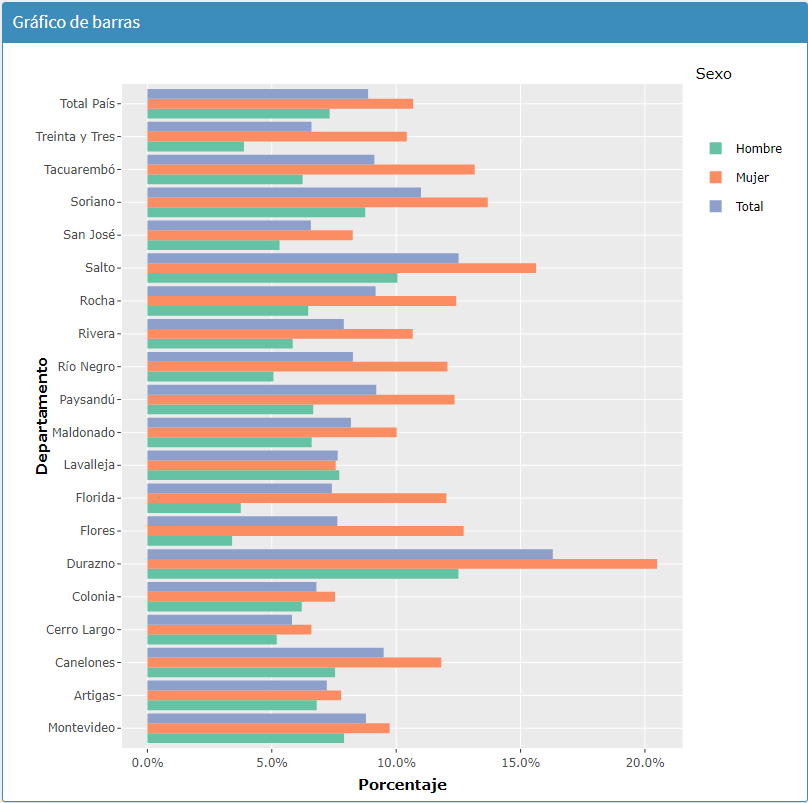
\includegraphics[width=1\textwidth]{img/barras.PNG}
\caption{Gráfico de barras de la tasa de desempleo a nivel departamental y de todo el país desagregando por sexo. \label{barras}}
\end{center}
\end{figure}

\begin{figure}[h]
\begin{center}
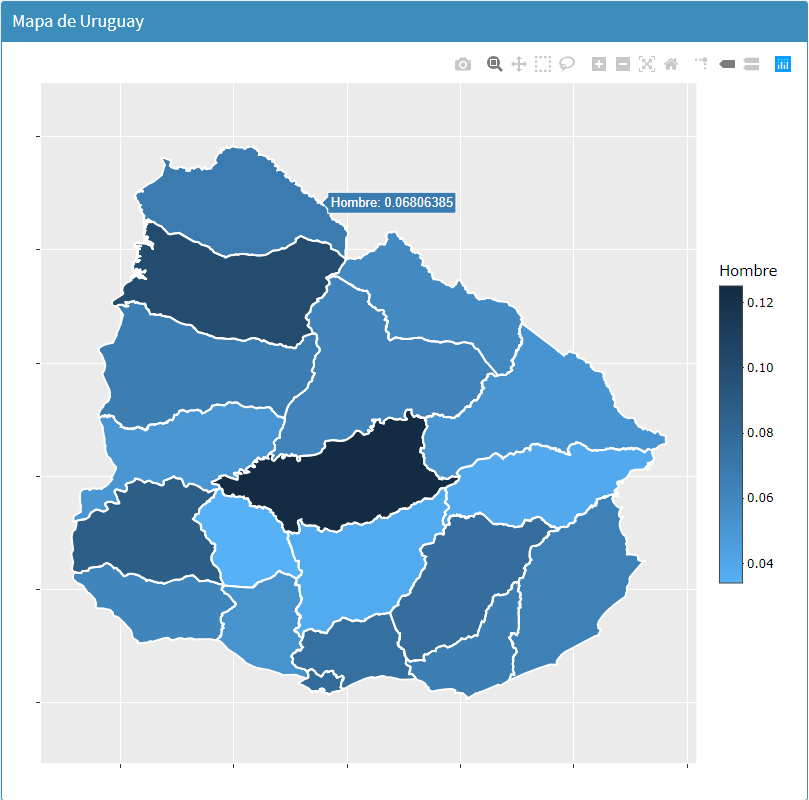
\includegraphics[width=1\textwidth]{img/Mapa.png}
\caption{Tasa de desempleo a nivel departamental para la categoría Hombres. \label{mapa}}
\end{center}
\end{figure}

Como se puede observar en la figura \ref{mapa}, al colocar el cursor sobre uno de los departamentos, el gráfico nos brinda el valor de la estimación para dicho departamento. Esto también es posible en el diagrama de barras presentado y es una de las ventajas del uso de gráficos interactivos creados con la librería \textit{plotly}.

Para el gráfico de mapa se debe seleccionar la categoría a graficar, en este caso las opciones son \textit{Hombre}, \textit{Mujer} o \textit{Total}. 

\begin{figure}[h]
\begin{center}
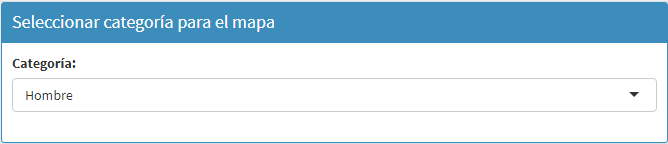
\includegraphics[width=1\textwidth]{img/cat_mapa.PNG}
\caption{Categorías para visualizar en el mapa. \label{catmapa}}
\end{center}
\end{figure}

En la segunda pestaña de esta sección se puede observar una tabla como la presentada en la figura \ref{tabl}, que contiene las estimaciones puntuales del indicador seleccionado, a nivel departamental y nacional.

\begin{figure}[htb]
\begin{center}
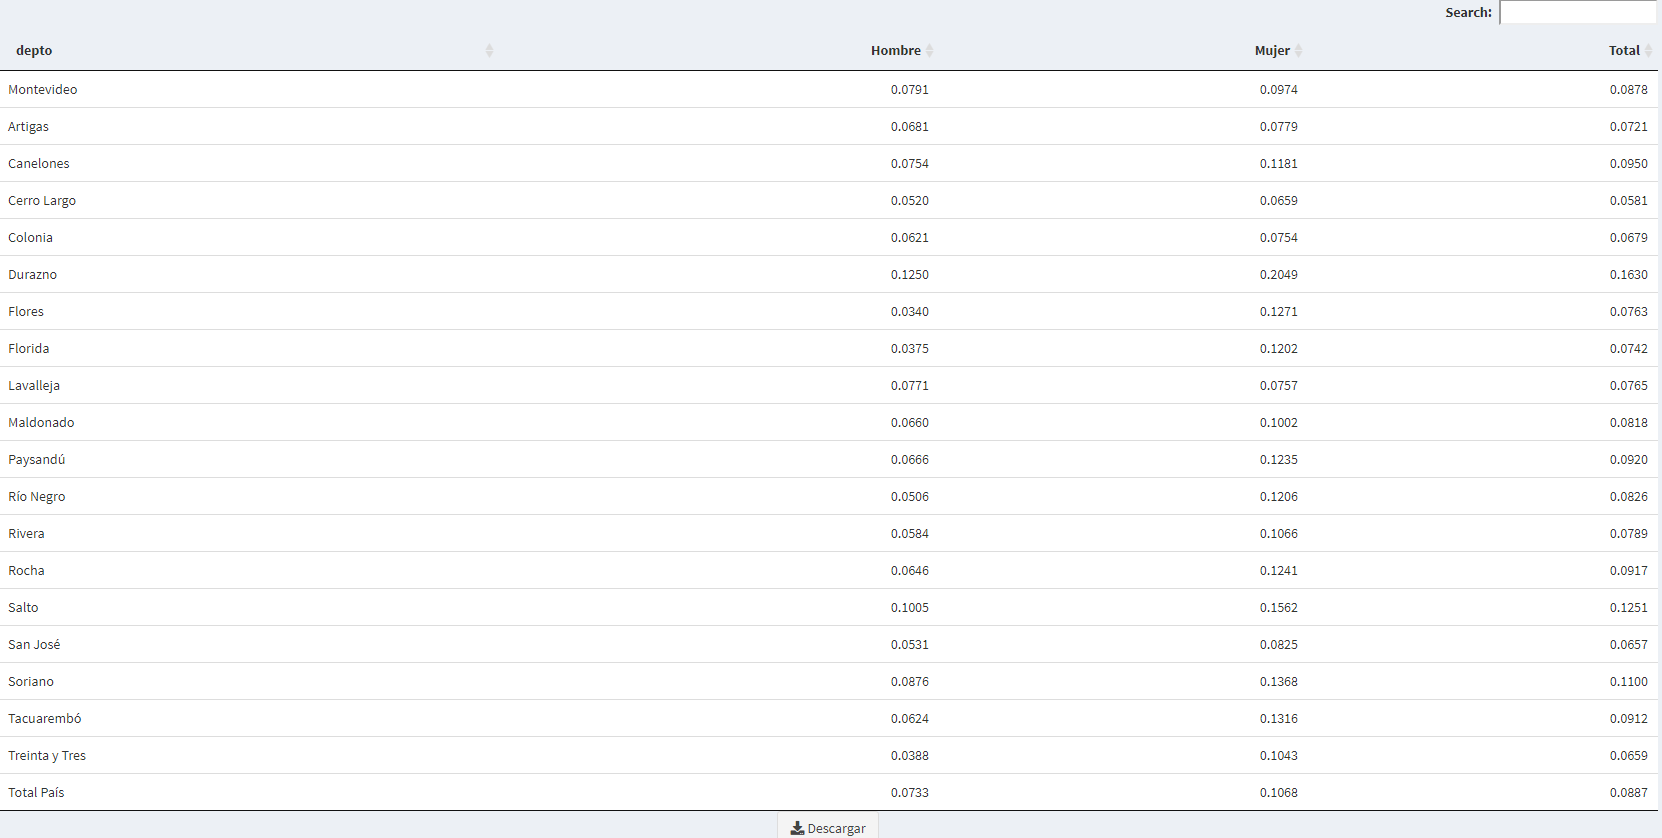
\includegraphics[width=1.2\textwidth]{img/tabla.PNG}
\caption{Tabla con las estimaciones puntuales de la tasa de desempleo para los 19 departamentos y para todo el país en el año 2019. \label{tabl}}
\end{center}
\end{figure}

Por último, en la pestaña \textit{IC}, se observan tablas con los límites de los intervalos de confianza al $95\%$ de las estimaciones anteriores.

\begin{figure}[htb]
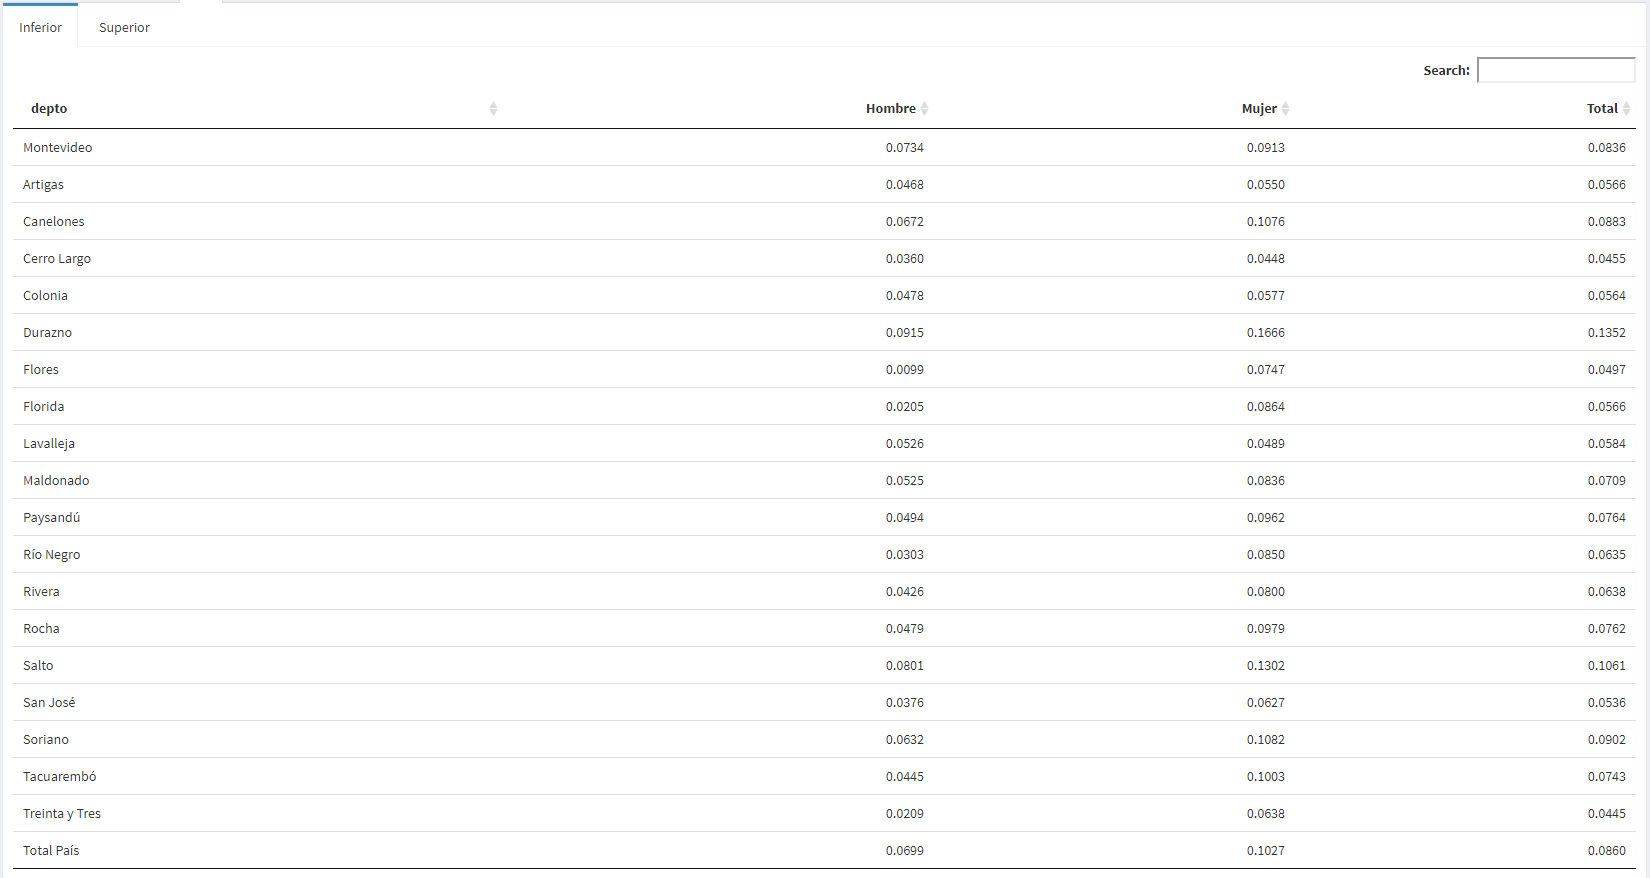
\includegraphics[width=1.2\textwidth]{img/inf.PNG}
\caption{Tabla con los límites inferiores de los intervalos de confianza al $95\%$ de las estimaciones puntuales de la tasa de desempleo para los 19 departamentos y para todo el país en el año 2019. \label{tablinf}}
\end{figure}

\begin{figure}[htb]
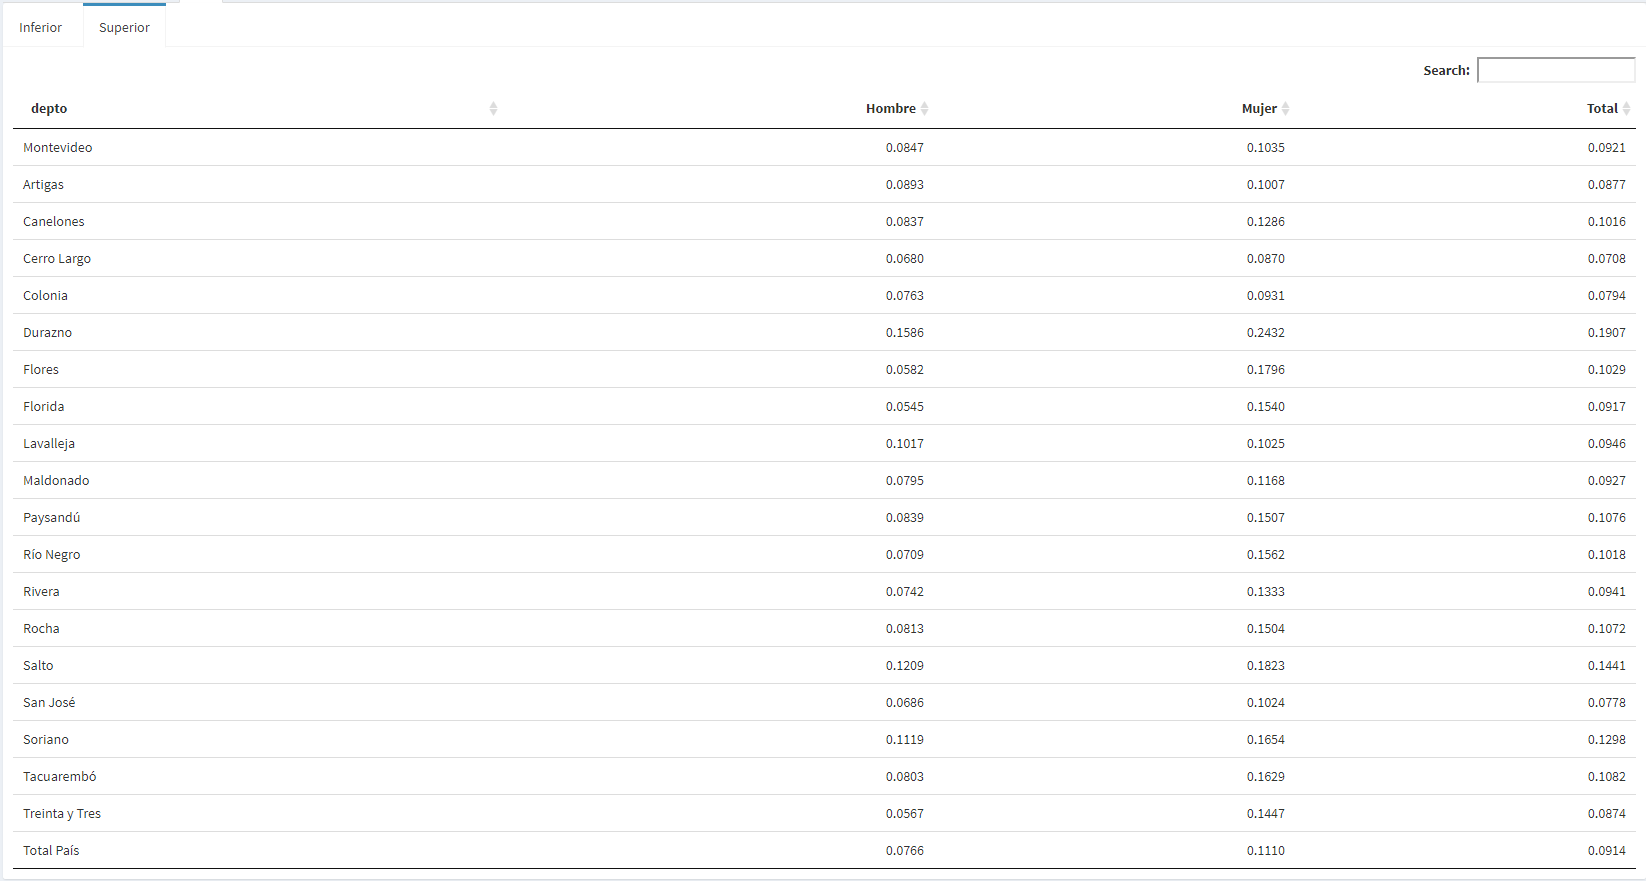
\includegraphics[width=1.2\textwidth]{img/sup.PNG}
\caption{Tabla con los límites superiores de los intervalos de confianza al $95\%$ de las estimaciones puntuales de la tasa de desempleo para los 19 departamentos y para todo el país en el año 2019. \label{tablsup}}
\end{figure}

\section{Hogares por presencia de lugar para cocinar \label{sec:hog}}

Por otra parte, el indicador \texttt{Hogares por presencia de lugar para cocinar} hace referencia a la proporción de hogares que cuentan con lugar apropiado para cocinar privado, con lugar apropiado compartido con otros hogares o que no cuentan con lugar apropiado y se calcula como $\frac{Numero\; de\; hogares\; segun \;presencia\;de\;lugar\;para\;cocinar}{Total \;hogares}$.

\begin{knitrout}
\definecolor{shadecolor}{rgb}{0.969, 0.969, 0.969}\color{fgcolor}\begin{kframe}
\begin{alltt}
\hlkwd{funcion9}\hlstd{(ph,} \hlstr{"d19"}\hlstd{,} \hlkwd{c}\hlstd{(}\hlstr{"dpto"}\hlstd{,} \hlstr{"Lugar privado"}\hlstd{,} \hlstr{"Compartido"}\hlstd{,}
         \hlstr{"No tiene"}\hlstd{),} \hlkwd{c}\hlstd{(}\hlnum{1}\hlstd{,}\hlnum{2}\hlstd{,}\hlnum{3}\hlstd{))}
\end{alltt}
\end{kframe}
\end{knitrout}

Este indicador se calcula sobre la base de hogares, se utiliza la \emph{funcion9}, el diseño \emph{ph}, filtro no tiene ya que se calcula sobre todos los hogares, la variable utilizada es \emph{d19} la cual es una variable presente en la ECH que hace referencia al lugar para cocinar y toma valor 1 cuando tiene lugar privado, 2 cuando es compartido con otros hogares y 3 cuando no tiene. Esta información es la que se le brinda a la función en los otros dos insumos.

En la app este indicador se encuentra en la sección \textit{Viviendas y hogares}, por lo que de igual manera que para el indicador anterior, se ingresa a la sección, se selecciona el indicador deseado y se observan los resultados.

\begin{figure}[htb]
\begin{center}
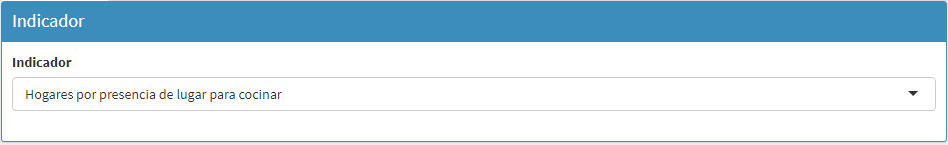
\includegraphics[width=1\textwidth]{img/indicador_hog.PNG}
\caption{Selección del indicador Hogares por presencia de lugar para cocinar. \label{ind2}}
\end{center}
\end{figure}

La diferencia en este indicador es que se presenta un gráfico de barras apiladas (\ref{barras2}) en lugar de agrupadas como era el caso de la tasa de desempleo.

\begin{figure}[htb]
\begin{center}
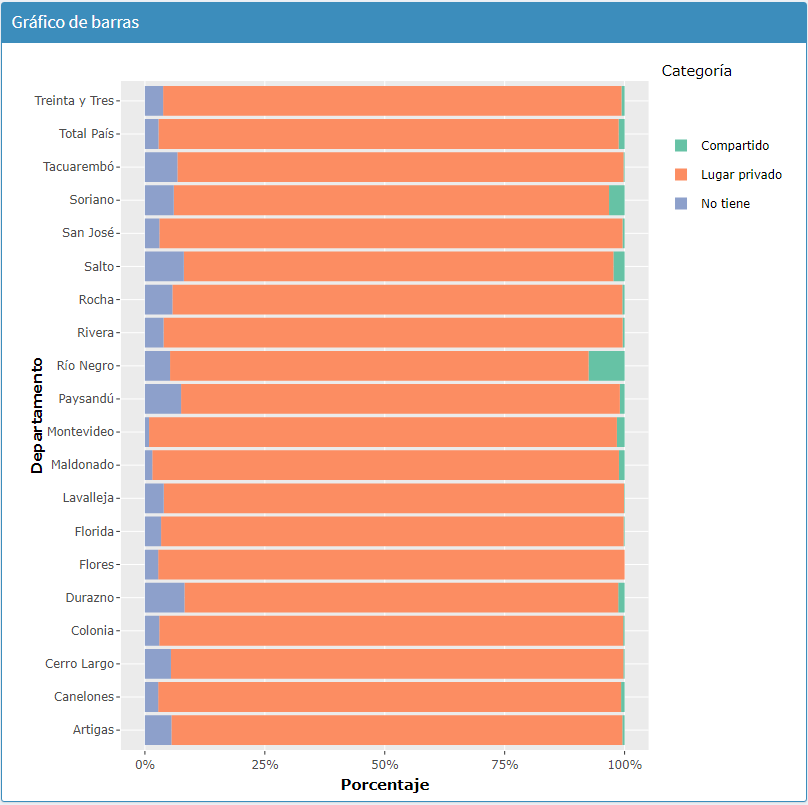
\includegraphics[width=1\textwidth]{img/Barras_hog.PNG}
\caption{Gráfico de barras de la proporción de hogares por presencia de lugar para cocinar por departamento. \label{barras2}}
\end{center}
\end{figure}

El gráfico de mapa es similar al presentado para la tasa de desempleo, donde también se puede seleccionar la categoría a visualizar. La visualización de las tablas de estimaciones puntuales e intervalos de confianza también son similares al caso del indicador anterior.

\begin{figure}[htb]
\begin{center}
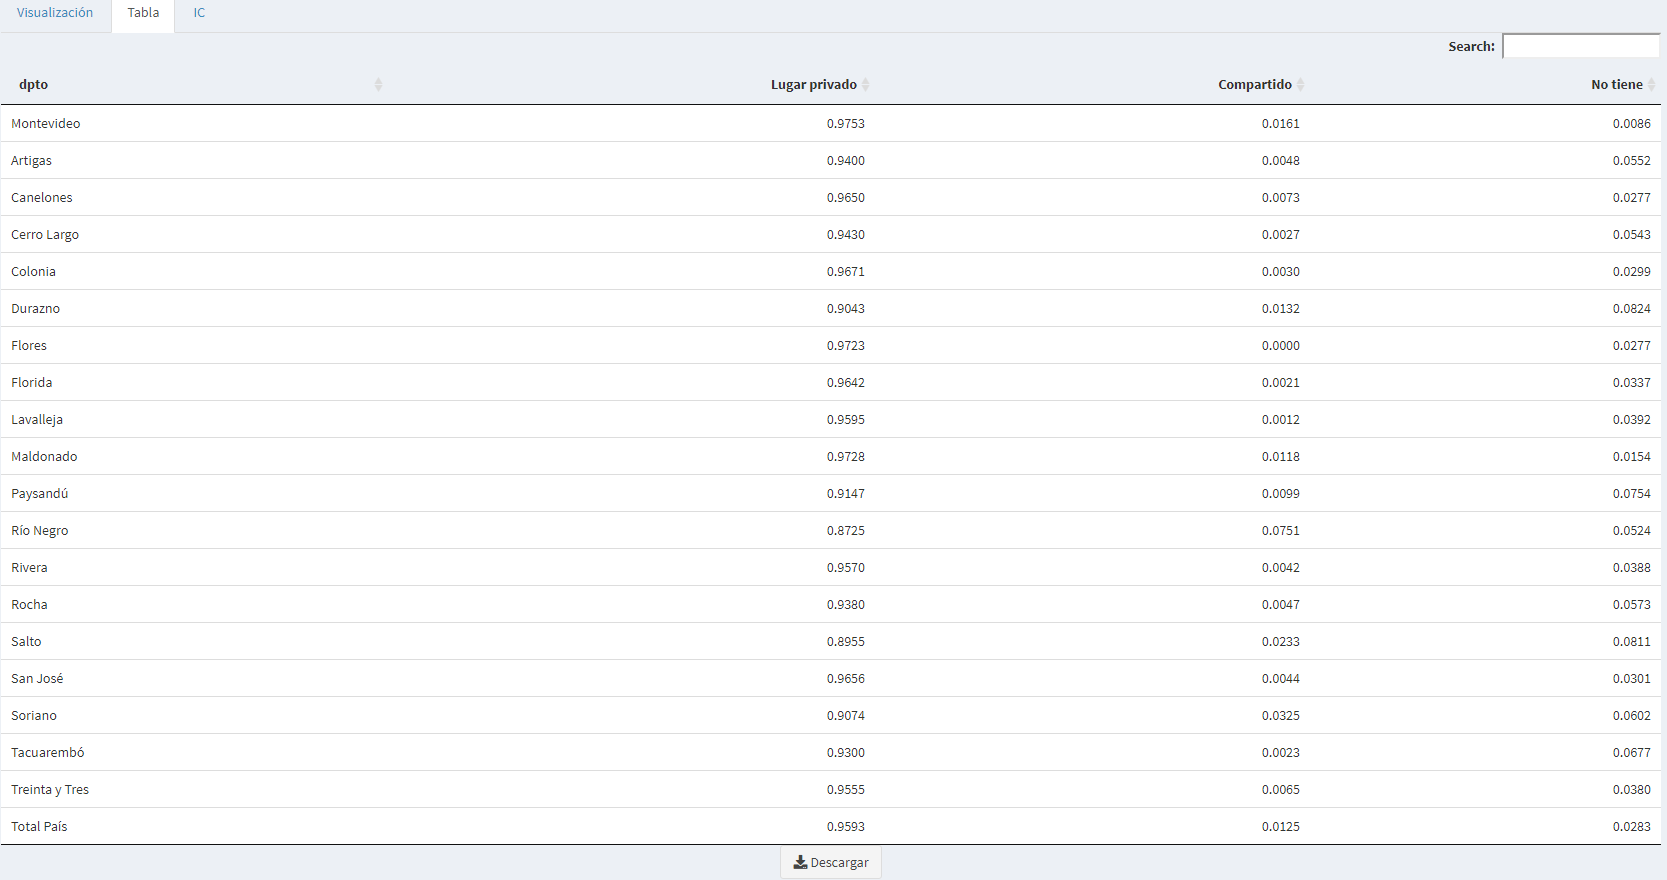
\includegraphics[width=1.2\textwidth]{img/tabla_hog.PNG}
\caption{Tabla con las estimaciones puntuales de la proporción de hogares por presencia de lugar para cocinar a nivel departamental y de todo el país en el año 2019. \label{tabl2}}
\end{center}
\end{figure}

\chapter{Discusión \label{cap:discu}}

La Encuesta Continua de Hogares permite obtener estimaciones sobre una gran cantidad de indicadores que abordan distintas dimensiones. Cada año el INE calcula una determinada cantidad de indicadores, en su mayoría a nivel de todo el país y desagregando en Montevideo e interior, añadiendo además algunas medidas de calidad de las estimaciones, como lo son los intervalos de confianza o coeficientes de variación.

Cualquier usuario puede obtener sus propias estimaciones puntuales sobre distintos indicadores a partir de la ECH, ya que para ello es necesario contar únicamente con los pesos muestrales, los cuales, se encuentran incluidos en las bases de datos públicas. Sin embargo resulta más complejo el poder obtener ciertas medidas de calidad de las estimaciones.

Como se mencionó en este trabajo, las medidas de calidad se obtienen a partir del cálculo de los errores estándar, y para el cálculo de estos se necesitan tener en cuenta todas las fuentes de variación que afectan las estimaciones. Se debe tener conocimiento sobre el proceso de selección de la muestra y contar con la disponibilidad de esta información en las bases públicas, en este caso la información sobre estratos y unidades primarias de muestreo.

Otra de las principales dificultades es la utilización de programas estadísticos para poder trabajar con estos datos. Es esta una de las principales ventajas que tiene la App de Shiny presentada en este trabajo, ya que no se necesita del conocimiento en ningún programa estadístico para su utilización. Esta App permite obtener en el momento, estimaciones puntuales sobre una batería de indicadores y sus respectivos intervalos de confianza, con solo cargar las bases de datos de la ECH del año que se desee. 

Otra de las ventajas que presenta esta aplicación, es el cálculo de una gran cantidad de indicadores en diferentes dominios, ya sean aperturas departamentales, variables como el sexo o diferentes tramos etarios.


\section{Limitaciones y trabajos a futuro \label{sec:lim}}

Una de las principales limitaciones que puede tener esta aplicación, es la dependencia sobre las variables de la ECH, es decir, el hecho de que si las variables utilizadas cambian de nombre o dejan de aparecer en encuestas de años próximos, la app debe ser modificada para su correcto funcionamiento.

Otras mejoras que puede tener la app son por ejemplo: gráficos para los intervalos de confianza; otras medidas de calidad de las estimaciones, como lo son coeficientes de variación o tamaños de muestra efectivos; obtener estimaciones en dominios más pequeños como por ejemplo separar a las capitales departamentales del resto del departamento; agregar más indicadores o dejar más libertad al usuario para que pueda calcular sus propios indicadores.

Independientemente de las posibles mejoras que pueda tener la app, siempre va a quedar a efectos del usuario el correcto uso de la misma y la correcta interpretación de los resultados.

%%%%%%%%%%%%%%%%%%%%%%%%%%%% BIBLIOGRAFíA %%%%%%%%%%%%%%%%%%%%%%%%%%%%%%%%%%%%%%%%%%%%

\bibliographystyle{apa}
\bibliography{TFGbiblo}


%%%%%%%%%%%%%%%%%%%%%%%%%%% ANEXO %%%%%%%%%%%%%%%%%%%%%%%%%%%%%%%%%%%%%%%%%%%%%%%%%%

\begin{appendix}

\chapter{Anexos} 

\section{Listado de indicadores \label{ane:ind}}

Se presenta el listado completo de los indicadores trabajados en la app.

% latex table generated in R 4.0.2 by xtable 1.8-4 package
% Wed Nov 11 12:53:42 2020
\begin{longtable}{p{2in}|p{1in}|p{0.5in}|p{1in}|p{0.5in}}
\caption{Listado de indicadores} \\ 
  \hline
Indicador & Categoría & Función & Desagregación & Base \\ 
  \hline
Tasa de analfabetismo en población de 15 años o más & Educación & 1 & Dpto - Sexo  & Personas \\ 
  Adolescentes de 12 a 17 años que asisten a establecimientos educativos & Educación & 1 & Dpto - Sexo  & Personas \\ 
  Personas mayores de 15 años que completaron media básica general o técnica & Educación & 1 & Dpto - Sexo  & Personas \\ 
  Personas de 18 años o más que completaron segundo ciclo de educación media & Educación & 1 & Dpto - Sexo  & Personas \\ 
  Población entre 25 y 65 años con estudios terciarios & Educación & 1 & Dpto - Sexo  & Personas \\ 
  Tasa neta de asistencia de 0 a 2 años en educación inicial & Educación & 1 & Dpto - Sexo  & Personas \\ 
  Tasa neta de asistencia de 3 a 5 años en educación preescolar & Educación & 1 & Dpto - Sexo  & Personas \\ 
  Tasa neta de asistencia de 6 a 11 años en educación primaria & Educación & 1 & Dpto - Sexo  & Personas \\ 
  Tasa neta de asistencia de 12 a 17 años en educación media & Educación & 1 & Dpto - Sexo  & Personas \\ 
  Personas mayores a 25 años por máximo nivel educativo alcanzado & Educación & 2 & Dpto - Sexo  & Personas \\ 
  Ocupados por máximo nivel educativo alcanzado & Educación & 2 & Dpto - Sexo & Personas \\ 
  Tasa de analfabetismo en mayores de 15 años & Educación & 3 & Dpto - Tramos de edad  & Personas \\ 
  Promedio de años de educación de las personas de 25 años o más & Educación & 6 & Dpto - Sexo  & Personas \\ 
  Tasa bruta de asistencia de 3 a 5 años en educación preescolar & Educación & 7 & Dpto & Personas \\ 
  Tasa bruta de asistencia de 6 a 11 años en educación primaria & Educación & 7 & Dpto  & Personas \\ 
  Tasa bruta de asistencia de 12 a 17 años en educación media & Educación & 7 & Dpto  & Personas \\ 
  Jóvenes de 14 a 24 años que no estudian ni trabajan & Educación / Mercado Laboral & 1 & Dpto - Sexo  & Personas \\ 
  Personas afiliadas a emergencias móviles & Salud & 1 & Dpto - Sexo  & Personas \\ 
  Personas afiliadas a emergencias móviles & Salud & 4 & Dpto - Tramos de edad  & Personas \\ 
  Personas por tipo de atención en salud & Salud & - & Dpto  & Personas \\ 
  Tasa de desempleo & Mercado Laboral & 1 & Dpto - Sexo  & Personas \\ 
  Subempleo & Mercado Laboral & 1 & Dpto - Sexo  & Personas \\ 
  Tasa de empleo & Mercado Laboral & 1 & Dpto - Sexo  & Personas \\ 
  Tasa de actividad & Mercado Laboral & 1 & Dpto - Sexo  & Personas \\ 
  Ocupados en establecimientos fuera de su departamento  & Mercado Laboral & 1 & Dpto - Sexo  & Personas \\ 
  Desocupados por última ocupación & Mercado Laboral & 2 & Dpto - Sexo  & Personas \\ 
  Ocupados por categoría de ocupación & Mercado Laboral & 2 & Dpto - Sexo  & Personas \\ 
  Tasa de actividad & Mercado Laboral & 5 & Dpto - Tramos de edad  & Personas \\ 
  Población total por condición de actividad & Mercado Laboral & - & Dpto - Sexo  & Personas \\ 
  Informalidad & Mercado Laboral / Ingresos y bienestar & 1 & Dpto - Sexo  & Personas \\ 
  Tasa de desempleo & Mercado Laboral / Ingresos y bienestar & 5 & Dpto - Tramos de edad  & Personas \\ 
  Tasa de empleo & Mercado Laboral / Ingresos y bienestar & 5 & Dpto - Tramos de edad  & Personas \\ 
  Personas en hogares en situación de pobreza & Ingresos y bienestar & 1 & Dpto - Sexo  & Personas \\ 
  Jóvenes entre 14 y 29 años en situación de pobreza & Ingresos y bienestar & 1 & Dpto - Sexo  & Personas \\ 
  Hogares con al menos 1 auto o camioneta & Ingresos y bienestar & 8 & Dpto  & Hogares \\ 
  Hogares en situación de pobreza & Ingresos y bienestar / Viviendas y hogares & 8 & Dpto  & Hogares \\ 
  Hogares con hacinamiento & Ingresos y bienestar / Viviendas y hogares & 8 & Dpto  & Hogares \\ 
  Personas con celular & Tecnología y comunicación & 1 & Dpto - Sexo  & Personas \\ 
  Utilización de computadora el último mes & Tecnología y comunicación & 1 & Dpto - Sexo  & Personas \\ 
  Personas que utilizan internet  & Tecnología y comunicación & 1 & Dpto - Sexo  & Personas \\ 
  Frecuencia de utilización de internet & Tecnología y comunicación & 2 & Dpto - Sexo & Personas \\ 
  Hogares con al menos una computadora del Plan Ceibal & Tecnología y comunicación & 8 & Dpto  & Hogares \\ 
  Hogares con conexión a internet & Tecnología y comunicación & 8 & Dpto  & Hogares \\ 
  Hogares con computadora o laptop & Tecnología y comunicación & 8 & Dpto  & Hogares \\ 
  Población por lugar de nacimiento & Demografía & 2 & Dpto - Sexo  & Personas \\ 
  Personas por lugar de residencia anterior & Demografía & 2 & Dpto - Sexo  & Personas \\ 
  Población por lugar de residencia hace 5 años & Demografía & 2 & Dpto - Sexo & Personas \\ 
  Hogares por tipo de evacuación del sistema sanitario & Viviendas y hogares & 9 & Dpto  & Hogares \\ 
  Hogares por presencia de lugar para cocinar & Viviendas y hogares & 9 & Dpto  & Hogares \\ 
  Hogares por presencia y uso de baño & Viviendas y hogares & 9 & Dpto  & Hogares \\ 
  Hogares por fuente de energía para iluminar & Viviendas y hogares & 9 & Dpto  & Hogares \\ 
  Hogares por origen de agua para beber y cocinar & Viviendas y hogares & 9 & Dpto  & Hogares \\ 
  Hogares por tipo de relación con la vivienda & Viviendas y hogares & - & Dpto & Hogares \\ 
  \hline
\end{longtable}



\section{Listado de variables \label{ane:var}}

Se presenta la tabla con las variables de la ECH que son utilizadas en la app.

% latex table generated in R 4.0.2 by xtable 1.8-4 package
% Wed Nov 11 12:53:42 2020
\begin{longtable}{p{1in}p{3.7in}p{1.3in}}
\caption{Listado de variables utilizadas en la app} \\ 
  \hline
Variables & Descripción & Base de datos \\ 
  \hline
dpto & Código correlativo del 1 al 19 comenzando por Montevideo y continuando alfabéticamente & Personas \\ 
  e26 & Sexo & Personas \\ 
  e27 & Edad & Personas \\ 
  e215 & Asistencia a magisterio o profesorado & Personas \\ 
  e218 & Asistencia a universidad o similar & Personas \\ 
  e221 & Asistencia a terciario no universitario & Personas \\ 
  e224 & Asistencia a postgrado & Personas \\ 
  pobpcoac & Condición de actividad económica & Personas \\ 
  e193 & Asistencia a educación preescolar & Personas \\ 
  e197 & Asistencia a educación primaria & Personas \\ 
  e201 & Asistencia a educación media & Personas \\ 
  e212 & Asistencia a educación técnica & Personas \\ 
  e51\_2 & Años aprobados en primaria común & Personas \\ 
  e51\_4 & Años aprobados en ciclo básico & Personas \\ 
  e51\_5 & Años aprobados en bachillerato & Personas \\ 
  e51\_6 & Años aprobados en bachillerato tecnológico & Personas \\ 
  e51\_7 & Años aprobados en educación técnica & Personas \\ 
  e51\_8 & Años aprobados en magisterio o profesorado & Personas \\ 
  e51\_9 & Años aprobados en universidad o similar & Personas \\ 
  e51\_10 & Años aprobados en terciario no universitario & Personas \\ 
  e51\_11 & Años aprobados en postgrado & Personas \\ 
  e51\_7\_1 & Exigencia para realizar curso de educación técnica & Personas \\ 
  e51\_3 & Años aprobados en primaria especial & Personas \\ 
  e236 & Lugar de residencia 5 años atrás & Personas \\ 
  numero & Número de identificación del hogar & Personas \\ 
  pesoano & Ponderador del año & Personas \\ 
  e238 & Asistencia a educación inicial & Personas \\ 
  e48 & Sabe leer y escribir & Personas \\ 
  e46 & Afiliación a emergencia móvil & Personas \\ 
  f82 & Aporte a caja de jubilaciones & Personas \\ 
  f80 & Trabajo en el departamento & Personas \\ 
  f116 & Ha trabajado antes & Personas \\ 
  f121 & Categoría de la ocupación (trabajos anteriores de no ocupados) & Personas \\ 
  f73 & Categoría de la ocupación & Personas \\ 
  pobre06 & Pobreza según metodología 2006 & Personas \\ 
  e62 & Utilización de internet en el último mes & Personas \\ 
  e61 & Utilización de microcomputador en el último mes & Personas \\ 
  e60 & Tenencia de teléfono celular & Personas \\ 
  e37 & Lugar de residencia inmediato luego del nacimiento & Personas \\ 
  e39 & Lugar de residencia anterior & Personas \\ 
  e45\_1 & ASSE & Personas \\ 
  e45\_2 & IAMC & Personas \\ 
  e45\_3 & Seguro médico privado & Personas \\ 
  e45\_4 & Hospital Policial/Militar & Personas \\ 
  e45\_5 & Área de salud del BPS & Personas \\ 
  e45\_6 & Policlínica municipal & Personas \\ 
  e45\_7 & Otro (salud) & Personas \\ 
  e65 & Frecuencia de utilización de internet & Personas \\ 
  subempleo & Trabajador subempleado & Personas \\ 
  d8\_1 & Tenencia de la vivienda & Hogares \\ 
  d25 & Total de personas del hogar & Hogares \\ 
  d9 & Habitaciones residenciales & Hogares \\ 
  d21\_18 & Automóvil o camioneta & Hogares \\ 
  d21\_16 & Conexión a internet & Hogares \\ 
  d21\_15 & Microcomputador & Hogares \\ 
  d21\_15\_1 & Algún microcomputador del Plan Ceibal & Hogares \\ 
  d16 & Evacuación del sistema sanitario & Hogares \\ 
  d18 & Fuente de energía para iluminar & Hogares \\ 
  d11 & Origen del agua & Hogares \\ 
  d19 & Lugar para cocinar & Hogares \\ 
  d15 & Uso de baño & Hogares \\ 
  upm\_fic & UPM & UPM y estratos \\ 
  estrato & Estratos & UPM y estratos \\ 
  \hline
\end{longtable}

\end{appendix}


\end{document}
